\section{Wechselkurse}
\subsection{Nominaler Wechselkurs}
Erhöht sich die inländische Geldmenge im Vergleich zur ausländischen dann steigt der nominale Wechselkurs. Dies ist eine Abwertung der inländischen Währung. Umgekehrt ist eine Erhöhung der ausländischen Geldmenge eine Aufwertung der inländischen Währung. 
\begin{equation*}
 e\quad (nominaler\quad Wechselkurs) = \frac{inländische\quad Währung}{ausländische\quad Währung}
\end{equation*}
\subsection{Realer Wechselkurs}
Bei den realen Wechselkursen werden die unterschiedlichen Preisniveaus im Inland und Ausland berücksichtigt.
\begin{equation*}
	r \quad(realer \quad Wechselkurs) = \frac{e \cdot p^{*} (Preis\quad Güterkorb \quad im\quad Ausland\quad in \quad ausländischer \quad Währung)}{p (Preis\quad Güterkorb\quad im\quad Inland\quad in\quad inländischer\quad Währung)}
\end{equation*}
\begin{itemize}
	\item Erhöhung inländische Geldmenge
	\subitem Nominaler Wechselkurs steigt sofort
	\subitem Langfristig ändert realer Wechselkurs nicht, da sich Preisniveau anpasst
\end{itemize}
\subsection{Fixe Wechselkurssysteme}
\begin{itemize}
	\item Berechnbarkeit des Wechselkurs
	\item Anbindung der eigenen Geldpolitik an stabilere Geldpolitik
	\item Vereinfacht Handelsbeziehungen
	\item Keine Möglichkeit zur Konjunktursteuerung
	\item Bei der EWS (Europäische Währungssystem) gibt es in den Ländern unterschiedliche Inflationsraten und Konjunkturzyklen, daher sind fixe Wechselkurse ein Problem
\end{itemize}
\subsection{Währungsunion}
\begin{itemize}
	\item In der Währungsunion sind die nominalen Wechselkurse fixiert durch eine Zentralbank
	\item Keine Wechselkursrisiko
	\item Erhöhung der Preistransparenz, da Güterkorbpreise direkt vergleichen werden können
	\item Falls die Länder trotzdem konjunkturell unterschiedlich sind sollte dies durch flexible Löhne, Preise, mobile Arbeitskräfte und ausgleichende Fiskalströme aufgefangen werden. 
	\item Dies funktioniert aber in der EWU (Europäischer Währungsunion) nicht
	\item Dadurch bauten sich makroökonomische Ungleichgewichte auf. Alle Mitgliedsstaaten konnten sich zu den gleichen Zinsen verschulden. Für die PIGS-Staaten war dies eine billige Verschuldung (Zinsen tief). Dies ist der Grund für die Eurokrise
\end{itemize}
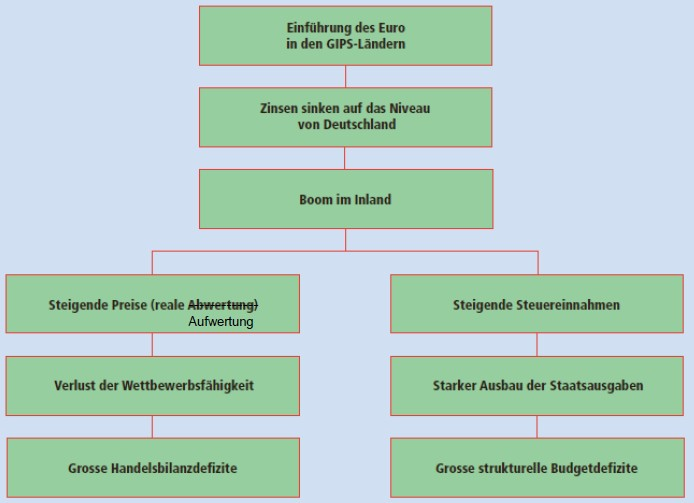
\includegraphics[width=0.8\linewidth]{images/eurokrise.jpg}